
\documentclass[12pt]{exam}
\usepackage{amsthm}
\usepackage{libertine}
%\usepackage[utf8]{inputenc}
\usepackage[margin=1in]{geometry}
\usepackage{amsmath,amssymb}
\usepackage{multicol}
\usepackage[shortlabels]{enumitem}
\usepackage{siunitx}
\usepackage{cancel}
\usepackage{graphicx}
\graphicspath{{./}}
\usepackage{pgfplots}
\usepackage{hyperref}
\usepackage{listings}
\usepackage{tikz}
\usepackage{minted}
\def\code#1{\texttt{#1}}
\usepackage{amssymb}
\usepackage{xcolor}
% for plotting
\usepackage{pgfplots}
\pgfplotsset{compat=1.16}
\usepackage{tikz}
\usetikzlibrary{arrows.meta}

\newcommand{\quotebox}[1]
{
  \begin{center}
    \fcolorbox{white}{blue!15!gray!15}{
      \begin{minipage}{0.7\linewidth}\vspace{10pt}
        \center
        \begin{minipage}{0.8\linewidth}{\space\Huge``}{\setlength{\parindent}{1.5em}#1}{\hspace{1.5em}\break\null\Huge\hfill''}
        \end{minipage}
        \smallbreak
      \end{minipage}
    }
\end{center}
}

%\DeclareUnicodeCharacter{2212}{-}


\let\oldemptyset\emptyset
\let\emptyset\varnothing

\hypersetup{
    colorlinks=true,
    linkcolor=blue,
    filecolor=magenta,      
    urlcolor=cyan,
    pdftitle={Overleaf Example},
    pdfpagemode=FullScreen,
    }
    
\urlstyle{same}

\pgfplotsset{width=10cm,compat=1.9}
\usepgfplotslibrary{external}
\tikzexternalize

\newcommand{\class}{Math 415} % This is the name of the course 
\newcommand{\examnum}{Homework-12} % This is the name of the assignment
\newcommand{\examdate}{Dec 12} % This is the due date
\newcommand{\timelimit}{}

\newcommand{\BO}{\mathcal{O}}




\begin{document}
\pagestyle{plain}
\thispagestyle{empty}

\noindent
\begin{tabular*}{\textwidth}{l @{\extracolsep{\fill}} r @{\extracolsep{6pt}} l}
\textbf{\class} & \textbf{Name:} & \textit{Zhenzhao Tu}\\ %Your name here instead, obviously 
\textbf{\examnum} &&\\
\textbf{\examdate} &&\\
\end{tabular*}\\
\rule[2ex]{\textwidth}{2pt}
% --


\section*{Problem 1}
Consider the quadratic map:
\[ x_{n+1} = x_n^2 + c \]
where $c$ is a constant. 

\begin{enumerate}
	\item Let $x_{n+1} = x_n$ we can find the fixed points are 
	\[ x = \frac{1 \pm \sqrt{1-4c}}{2} \]
	Then we find the $r$ with $|f'(x)| < 1$. Thus we have when $-3/4 < c<1/4$, the $x = (1-\sqrt{1-4c})/2$ is stable, and $x = (1+\sqrt{1-4c})/2$ is unstable. When $c > \frac{1}{4}$, the two fixed points are not real.	

	\item Based on the result of (a), we can plot the bifurcation diagram as follows:

		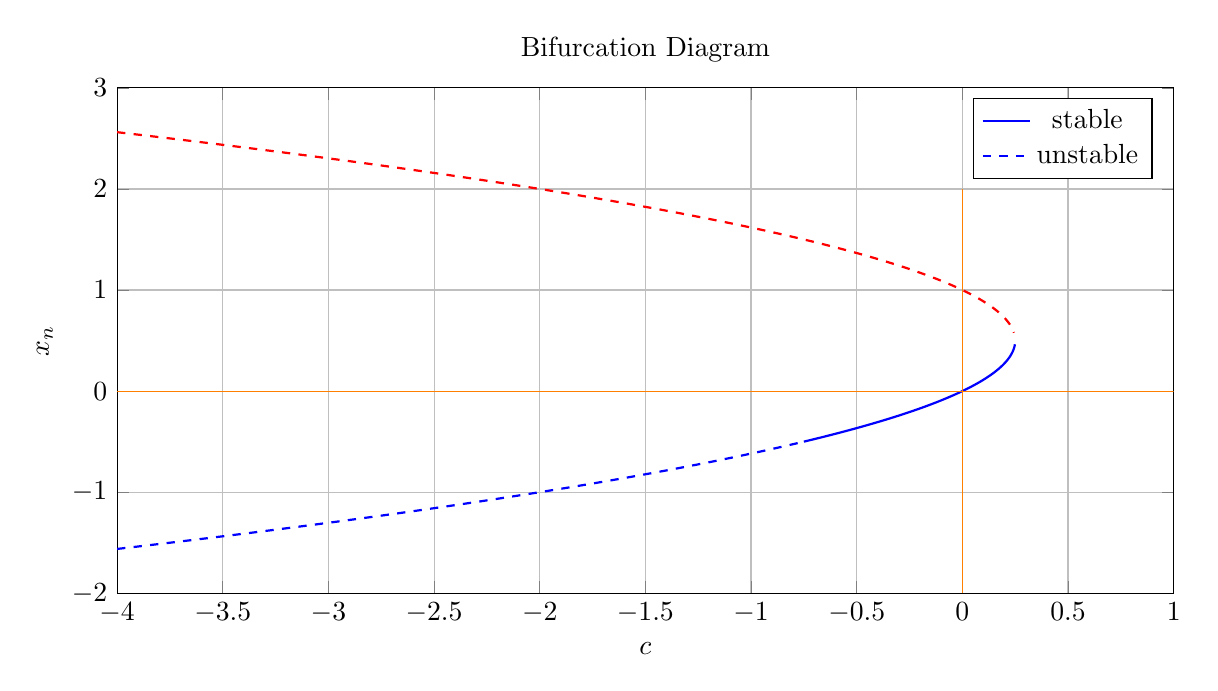
\begin{tikzpicture}
		\begin{axis}[
			title = {Bifurcation Diagram},
			xlabel = {$c$},
			ylabel = {$x_n$},
			xmin = -4, xmax = 1,
			ymin = -2, ymax = 3,
			grid = major,
			width = 15cm,
			height = 8cm,
			]
			% add the curve y=\frac{1-\sqrt{1-4c}}{2}
			\addplot[blue, thick, domain=-3/4:1/4, samples=700] {0.5*(1-sqrt(1-4*x))};
			% add the curve y=\frac{1-\sqrt{1-4c}}{2} from -4 to -3/4 with dashed line
			\addplot[blue, thick, dashed, domain=-4:-3/4, samples=700] {0.5*(1-sqrt(1-4*x))};
			% add the curve y=\frac{1+\sqrt{1-4c}}{2} from 1/4 to -4
			\addplot[red, thick, dashed, domain=-4:1/4, samples=700] {0.5*(1+sqrt(1-4*x))};
		
			% add horizontal line x=0
			\addplot[orange, domain=-4:1, samples=100] {0};
			% add vertical line y=0
			\addplot[orange, domain=-4:1, samples=100] coordinates {(0,-2) (0,2)};
			
			

			\legend{$\text{stable}$, $\text{unstable}$}
		\end{axis}
		\end{tikzpicture}

		Thus we know that at $c=1/4$ there is a saddle-node bifurcation.

	\item For stable $2$-cycle, we need to set $x^* = f^2(x^*)$, whichs is $x^* = x^4 + 2cx^2 + c^2 - x^* = 0$. We have two fixed points $x^* = \frac{1 \pm \sqrt{1-4c}}{2}$ which can be represented as $p,q$. Thus we have
		\[ x^4 + 2cx^2 + c^2 - x^* = (x-p)(x-q)(x^2+bx+c) = 0 .\]
		Then we can use polynomial division to get $x^2+bx+c$:
		\[ (x^2 + x+ c+1)(x-p)(x-q) = 0 .\]
		Thus we have last two fixed points $x^* = \frac{-1 \pm \sqrt{-3-4c}}{2}$ which can be represented as $r,s$. Thus we have
		\begin{align}
			p &= \frac{1 + \sqrt{1-4c}}{2} \\
			q &= \frac{1 - \sqrt{1-4c}}{2} \\
			r &= \frac{-1 + \sqrt{-3-4c}}{2} \\
			s &= \frac{-1 - \sqrt{-3-4c}}{2} 
		\end{align}
		Then let's find the stability of $2$-cycle. The derivative of $f(x)$ is $f'(x) = 2x$. Thus we have
		\[ f'(r)f'(s) = \frac{4}{4}(-1 + \sqrt{-3-4c})(-1 - \sqrt{-3-4c}) = 4c+4 .\]
		So, linearly stable for $|4c+4| < 1$ is $c \in (-5/4, -3/4)$.
		
	\item For detials of the bifurcation diagram, we can see below:

		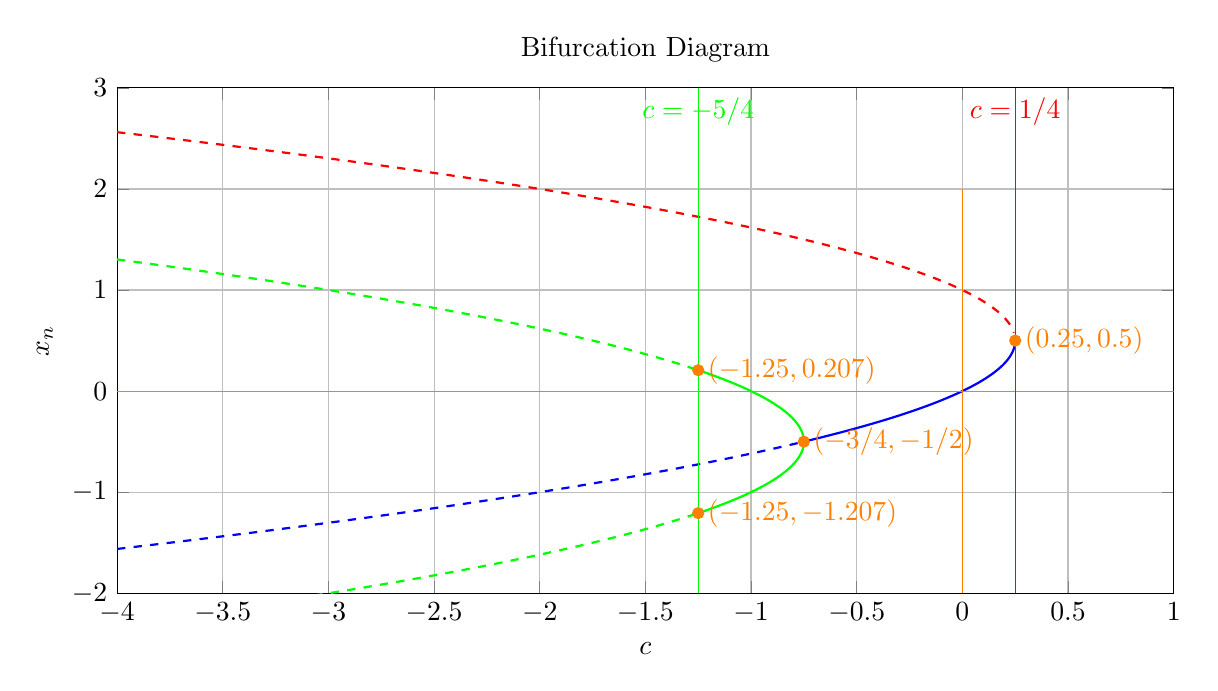
\begin{tikzpicture}
		\begin{axis}[
			title = {Bifurcation Diagram},
			xlabel = {$c$},
			ylabel = {$x_n$},
			xmin = -4, xmax = 1,
			ymin = -2, ymax = 3,
			grid = major,
			width = 15cm,
			height = 8cm,
			]
			% add the curve y=\frac{1-\sqrt{1-4c}}{2}
			\addplot[blue, thick, domain=-3/4:1/4, samples=700] {0.5*(1-sqrt(1-4*x))};
			% add the curve y=\frac{1-\sqrt{1-4c}}{2} from -4 to -3/4 with dashed line
			\addplot[blue, thick, dashed, domain=-4:-3/4, samples=700] {0.5*(1-sqrt(1-4*x))};
			% add the curve y=\frac{1+\sqrt{1-4c}}{2} from 1/4 to -4
			\addplot[red, thick, dashed, domain=-4:1/4, samples=700] {0.5*(1+sqrt(1-4*x))};

			% add horizontal line x=0
			\addplot[orange, domain=-4:1, samples=100] {0};
			% add vertical line y=0
			\addplot[orange, domain=-4:1, samples=100] coordinates {(0,-2) (0,2)};
			% add the curve y=\frac{-1+\sqrt{-3-4c}}{2}
			\addplot[green, thick, domain=-5/4:-3/4, samples=700] {0.5*(-1+sqrt(-3-4*x))};
			% add the curve y=\frac{-1+\sqrt{-3-4c}}{2} from -4 to -5/4 with dashed line
			\addplot[green, thick, dashed, domain=-4:-5/4, samples=700] {0.5*(-1+sqrt(-3-4*x))};
			% add the curve y=\frac{-1-\sqrt{-3-4c}}{2}
			\addplot[green, thick, domain=-5/4:-3/4, samples=700] {0.5*(-1-sqrt(-3-4*x))};
			% add the curve y=\frac{-1-\sqrt{-3-4c}}{2} from -4 to -5/4 with dashed line
			\addplot[green, thick, dashed, domain=-4:-5/4, samples=700] {0.5*(-1-sqrt(-3-4*x))};
			% add vertical line y=-5/4 in green and with label "c=-5/4"
			\addplot[green, domain=-2:1, samples=100] coordinates {(-5/4,-2) (-5/4,3)} node[below] {$c=-5/4$};
			
			% add vertical line y=1/4 in red and with label "c=1/4"
			\addplot[red, domain=-2:1, samples=100] coordinates {(1/4,-2) (1/4,3)} node[below] {$c=1/4$};
			% add a point at (1/4,1/2) with label "(0.25,0.5)"
			\addplot[mark=*, orange] coordinates {(1/4,1/2)} node[right] {$(0.25,0.5)$};
			% add a point at (-0.75,-0.5) with label "$(-3/4,-1/2)$"
			\addplot[mark=*, orange] coordinates {(-0.75,-0.5)} node[right] {$(-3/4,-1/2)$};
			% add a point at (-1.25,0.207) with label "$(-1.25,0.207)$"
			\addplot[mark=*, orange] coordinates {(-1.25,0.207)} node[right] {$(-1.25,0.207)$};
			% add a point at (-1.25,-1.207) with label "$(-1.25,-1.207)$"
			\addplot[mark=*, orange] coordinates {(-1.25,-1.207)} node[right] {$(-1.25,-1.207)$};
			%\legend{$\text{stable}$, $\text{unstable}$, $\text{stable}$}
		\end{axis}
		\end{tikzpicture}

	\item Given $y_n = ax_n + b$, we have $y_{n+1} = ax_{n+1} +b$ then substitute the logistic map $y_{n+1} = ry_n(1-y_n)$. Then we have
		\begin{align*}
			ax_{n+1} + b &= r(ax_n + b)(1-(ax_n+b)) \\
			ax_{n+1} &= r(ax_n + b)(1-(ax_n+b)) - b \\
			x_{n+1} &= \frac{r(ax_n + b)(1-(ax_n+b)) - b}{a} 
		\end{align*}
		Then we want to match the form of the quadratic map $x_{n+1} = x_n^2 + c$. Thus we have
		\[ x_{n+1} = -arx_n^2 + (r-2br)x + \frac{rb-rb^2-b}{a} .\]
		Then we can match the coefficients to get
		\begin{align}
			-ar &= 1 \\
			r-2br &= 0 \\
			\frac{rb-rb^2-b}{a} &= c
		\end{align}
		Thus we have
		\[ b = \frac{1}{2}, \quad a = -\frac{1}{r}, \quad c = \frac{r}{2} - \frac{r^2}{4}.\]
		



\end{enumerate}

\section*{Problem 2}
Consider the decimal shift map which maps $[0, 1]$ onto $[0, 1]$:
\[ x_{n+1} = 10x_n \quad (\text{mod } 1) .\]
\begin{enumerate}
	\item By listing out every $x_n$ we can find that there is a period relationship between every $0.1$ distance. They such rate is $10$ and the period is $0.1$. Thus we can use this infomation to draw the graph

		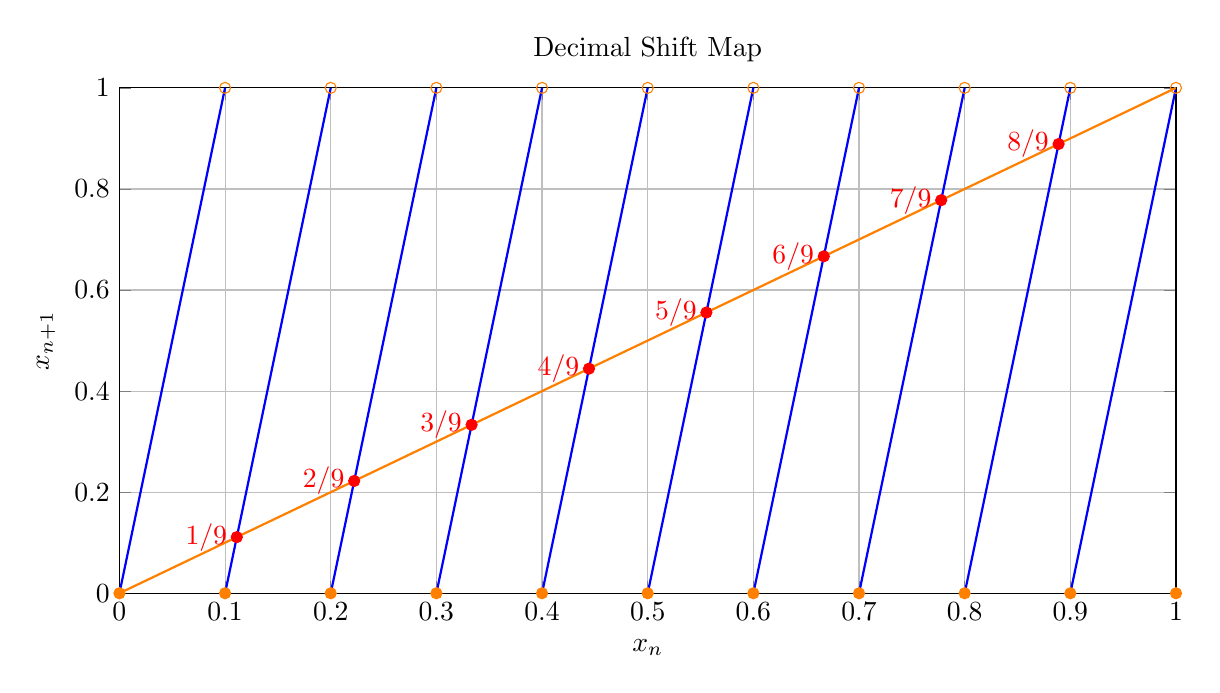
\begin{tikzpicture}
		\begin{axis}[
			title = {Decimal Shift Map},
			xlabel = {$x_n$},
			ylabel = {$x_{n+1}$},
			xmin = 0, xmax = 1,
			ymin = 0, ymax = 1,
			grid = major,
			width = 15cm,
			height = 8cm,
			]

			% add y = 10x from 0 to 0.1
			\addplot[blue, thick, domain=0:0.1, samples=700] {10*x};
			% add y = 10(x-0.1) from 0.1 to 0.2
			\addplot[blue, thick, domain=0.1:0.2, samples=700] {10*(x-0.1)};
			% add y = 10(x-0.2) from 0.2 to 0.3
			\addplot[blue, thick, domain=0.2:0.3, samples=700] {10*(x-0.2)};
			% add y = 10(x-0.3) from 0.3 to 0.4
			\addplot[blue, thick, domain=0.3:0.4, samples=700] {10*(x-0.3)};
			% add y = 10(x-0.4) from 0.4 to 0.5
			\addplot[blue, thick, domain=0.4:0.5, samples=700] {10*(x-0.4)};
			% add y = 10(x-0.5) from 0.5 to 0.6
			\addplot[blue, thick, domain=0.5:0.6, samples=700] {10*(x-0.5)};
			% add y = 10(x-0.6) from 0.6 to 0.7
			\addplot[blue, thick, domain=0.6:0.7, samples=700] {10*(x-0.6)};
			% add y = 10(x-0.7) from 0.7 to 0.8
			\addplot[blue, thick, domain=0.7:0.8, samples=700] {10*(x-0.7)};
			% add y = 10(x-0.8) from 0.8 to 0.9
			\addplot[blue, thick, domain=0.8:0.9, samples=700] {10*(x-0.8)};
			% add y = 10(x-0.9) from 0.9 to 1
			\addplot[blue, thick, domain=0.9:1, samples=700] {10*(x-0.9)};

			% add hollow circle at (0.1,1)
			\addplot[mark=o, orange] coordinates {(0.1,1)};
			% add hollow circle at (0.2,1)
			\addplot[mark=o, orange] coordinates {(0.2,1)};
			% add hollow circle at (0.3,1)
			\addplot[mark=o, orange] coordinates {(0.3,1)};
			% add hollow circle at (0.4,1)
			\addplot[mark=o, orange] coordinates {(0.4,1)};
			% add hollow circle at (0.5,1)
			\addplot[mark=o, orange] coordinates {(0.5,1)};
			% add hollow circle at (0.6,1)
			\addplot[mark=o, orange] coordinates {(0.6,1)};
			% add hollow circle at (0.7,1)
			\addplot[mark=o, orange] coordinates {(0.7,1)};
			% add hollow circle at (0.8,1)
			\addplot[mark=o, orange] coordinates {(0.8,1)};
			% add hollow circle at (0.9,1)
			\addplot[mark=o, orange] coordinates {(0.9,1)};
			% add hollow circle at (1,1)
			\addplot[mark=o, orange] coordinates {(1,1)};

			% add circle at (0.1,0)
			\addplot[mark=*, orange] coordinates {(0.1,0)};
			% add circle at (0.2,0)
			\addplot[mark=*, orange] coordinates {(0.2,0)};
			% add circle at (0.3,0)
			\addplot[mark=*, orange] coordinates {(0.3,0)};
			% add circle at (0.4,0)
			\addplot[mark=*, orange] coordinates {(0.4,0)};
			% add circle at (0.5,0)
			\addplot[mark=*, orange] coordinates {(0.5,0)};
			% add circle at (0.6,0)
			\addplot[mark=*, orange] coordinates {(0.6,0)};
			% add circle at (0.7,0)
			\addplot[mark=*, orange] coordinates {(0.7,0)};
			% add circle at (0.8,0)
			\addplot[mark=*, orange] coordinates {(0.8,0)};
			% add circle at (0.9,0)
			\addplot[mark=*, orange] coordinates {(0.9,0)};
			% add circle at (1,0)
			\addplot[mark=*, orange] coordinates {(1,0)};
			% add circle at (0,0)
			\addplot[mark=*, orange] coordinates {(0,0)};

			% add y=x line
			\addplot[thick, orange, domain=0:1, samples=100] {x};


			% add red circle at (1/9, 1/9) with label "1/9"
			\addplot[mark=*, red] coordinates {(1/9, 1/9)} node[left] {$1/9$};
			% add red circle at (2/9, 2/9) with label "2/9" 
			\addplot[mark=*, red] coordinates {(2/9, 2/9)} node[left] {$2/9$};
			% add red circle at (3/9, 3/9) with label "3/9"
			\addplot[mark=*, red] coordinates {(3/9, 3/9)} node[left] {$3/9$};
			% add red circle at (4/9, 4/9) with label "4/9"
			\addplot[mark=*, red] coordinates {(4/9, 4/9)} node[left] {$4/9$};
			% add red circle at (5/9, 5/9) with label "5/9"
			\addplot[mark=*, red] coordinates {(5/9, 5/9)} node[left] {$5/9$};
			% add red circle at (6/9, 6/9) with label "6/9"
			\addplot[mark=*, red] coordinates {(6/9, 6/9)} node[left] {$6/9$};
			% add red circle at (7/9, 7/9) with label "7/9"
			\addplot[mark=*, red] coordinates {(7/9, 7/9)} node[left] {$7/9$};
			% add red circle at (8/9, 8/9) with label "8/9"
			\addplot[mark=*, red] coordinates {(8/9, 8/9)} node[left] {$8/9$};




		\end{axis}
		\end{tikzpicture}

	\item The fixed points has been pointed out in (a) grpah. They are $0.aaaaaaa...$ where $a \in \{0,1,2,3,4,5,6,7,8\}$. Thus we have $9$ fixed points. Since $f'(x) =10 >1$, all the fixed points are unstable. 

	\item For a period-$p$ cycle where $p>1$, we can find a $x_n = x_{n+p}$ such this condition. Thus we have
		\[ 0.(a_0a_1 \dots a_{p})...(a_0a_1 \dots a_{p})...(a_0a_1 \dots a_{p}) \]
		Then we can find the period-$p$ cycle is $0.a_0a_1...a_{p}$. Thus we have
		\[ x_{n+p} = 10^{p}x_n \quad (\text{mod } 1) .\]
		Since $f'(x) = 10^{p} > 1$, all the period-$p$ cycles are unstable.
	
	\item When $x_n$ is an irrational number, then we know that $x_n$ is aperiodic. For example $\pi$.
	
	\item The Liapunov exponent is defined as
		\[ \lambda = \lim_{n\to\infty} \frac{1}{n} \sum_{i=0}^{n-1} \ln |f'(x_i)| .\]
		Then we can calculate the Liapunov exponent for the decimal shift map. Since $f'(x) = 10$, we have
		\[ \lambda = \lim_{n\to\infty} \frac{1}{n} \sum_{i=0}^{n-1} \ln |10| = \ln 10 .\]
		Thus we have $\lambda = \ln 10 \approx 2.30$. Thus we know that the decimal shift map is chaotic.

\end{enumerate}

\end{document}

